\chapter{什么是QFT?}
\section{为什么要学习量子场论}
量子场论包含无穷多自由度,比单粒子非相对论要复杂很多。在非相对论情况,我们比较熟悉的是谐振子的情况:$H=\frac{\textbf{p}^{2}}{2m}+\frac{1}{2}m^{2}\omega^{2}x^{2}$,
其能级为$E_{n}=(n+\frac{1}{2})\hbar\omega$,n=1,2,3 $\cdots$。
量子场论可以看成是无穷多个谐振子的联合,因此即使我们对于单粒子的谐振子情况已经了解得比较透彻了,但是在场论里面对无穷多谐振子耦合在一起的情况,仍然需要面对极其困难的复杂性。

量子场论之所以重要是因为其具有极其广泛的应用,可以应用在物理学的很多分支当中。尽管其发源于高能物理,但如今在高能物理、核物理、原子物理、凝聚态物理、宇宙学等方面仍有重要的作用,从最微观到最宏观都有发挥其作用的空间。本课程主要关注量子场论在高能物理中的应用。

量子场论具有非常强大的预言能力。电子的反常磁矩是人类在自然科学中理论和实验吻合得最好的例子之一,QED的预言与实验测量到小数点后第九位数字仍然是一致的。

20世纪初发展起来的狭义相对论和量子力学可以看作是牛顿体系在两个不同纬度的推广,前者成功描述了运动速度可以与光速相比的系统,后者成功描述了角动量与普朗克常数可以相比的微观系统,但这两大理论内部是不自洽的,为了能够使狭义相对论($E=m c^{2}$)与量子力学($i \hbar \frac{\partial}{\partial t}\psi=\hat{H}\psi$)统一起来,早期人们进行过许多尝试,但结果是人们经过多年的努力后发现,简单的把薛定谔方程改成协变的形式会遇到各种问题,唯一自洽的可能是抛弃固定粒子数的概念,引入量子场论的框架。
\begin{center}
QFT=SQ+QM
\end{center}

为什么学习粒子物理需要学习场论?两者之间有什么关系?Faraday提出了场的概念,Einstein提出了光量子的概念。可以认为,粒子是场激发对应的量子,即粒子首先是一个量子。考虑一个池塘,其中的水面是静止的,往池塘里扔进一个石子扰动水面,会在水面上出现涟漪,如果我们认为水是场,那么水波就是场激发产生的粒子。类似地,光子可以认为是电磁场激发后,具有确定能量和动量的水波,它具有粒子的属性。今后我们将使用这种图像理解许多粒子,如Higgs粒子,它可以通过激发一个标量场得到,电子则可以通过激发连续分布的电子场得到。

量子场论可以用来描述粒子数改变的过程。非相对论量子力学中粒子数是严格守恒的,但在真实的世界中有很多复杂的现象,难以使用量子力学来描述,在高能物理中,粒子能量较高,可以衰变成其他粒子,而在低能的情况,如凝聚态物理中,其能量小于电子的静止能量,因而无法产生新的电子,这里我们主要关注相对论性的量子场论。
以下考虑两个例子。

第一个例子是原子的自发辐射。考虑一个处于第一激发态的粒子,它有一定的几率会回到基态,假设第一激发态与基态的能量差是$\Delta E$,由于能量守恒,这一过程会释放出一个能量为$\Delta E$的光子$\gamma$,即$e^{-} \longrightarrow e^{-}+\gamma$。这一过程是一个粒子数改变的过程,其初态只有一个电子,而末态则有一个电子和一个光子。量子力学无法解释这一个光子从何而来,从场论的角度,光子可以认为是电磁场的激发态对应的量子,由于电磁场与电子场进行相互作用,从而有一定的几率电子场可以把电磁场激发出一个光子。

第二个例子是原子核的$\beta$衰变。这是一个由弱相互作用引导的过程:$n \longrightarrow p+e^{-}+\overline{\nu}_{e}$,其中涉及到了四种不同的粒子产生和湮灭的过程。历史上,1930sFeimi引入了4粒子相互作用来解释这一现象。
\section{历史回顾——相对论性量子力学}
描写固定粒子数的相对论性粒子的相对论性量子力学始于de Broglie、Schr$\ddot{\rm{o}}$dinger、Klein、Gordon、Dirac等人。这一理论在早期获得了一定的成功,但最终遇到了三个困难,必须让位于量子场论。这三个困难是:
\begin{itemize}
    \item 负能解问题,会导致不存在稳定的真空
    \item 负几率问题,统计诠释中$\rho=|\psi(x)|^{2}$代表粒子出现在某点的几率,其必须正定,但是在相对论性量子力学中这一正定性不再成立,意味着我们必须放弃波函数的几率诠释
    \item 因果性破坏
\end{itemize}

下面我们来谈论一些具体的历史。
Einstein光量子假设(1905):光子能量是一份一份的,$E=h\nu=\hbar \omega$,$\nu$是频率,$\omega$是角频率。

de Broglie物质波假设(1923):受狭义相对论以及光量子假设的启发,考虑一个自由电子,其四动量为$p^{\mu}=(\frac{{E}}{c},\vec{p})$,对应的物质波的波函数为平面波形式\footnote{这里采用的度规为$g^{\mu\nu}=diag(-1,1,1,1)$,今后如不特殊说明我们采用$g^{\mu\nu}=diag(1,-1,-1,-1)$}\footnote{今后所有的四矢量均用不带箭头的量表示,三分量矢量用带箭头的量表示}
\begin{equation}
    e^{ikx}=e^{ik^{\mu}x_{\mu}}e^{i\vec{k}\cdot \vec{x}-i \omega t}
\end{equation}
其中$k^{\mu}=(\frac{\omega}{c},\vec{k})$,$x^{\mu}=(ct,\vec{x})$,为了使得相位是Lorentz不变量,我们必须有$k^{\mu}$是四矢量。对于自由粒子的简单情况,电子自身的四动量$p^{\mu}$与$k^{\mu}$不应当是独立的,它们之间应该存在一定的比例关系,$k^{\mu}\propto p^{\mu}$。根据光量子假设,我们有$E=\hbar \omega$,因此$p^{\mu}=\hbar k^{\mu}$,写成分量的形式有$E=\hbar \omega,\vec{p}=\hbar \vec{k}=\frac{h}{\lambda}$。
对于一个物质粒子,它对应的物质波的粒子属性是由粒子的四动量$p$刻画的,波的属性是由波矢$k$刻画的,上面的结果告诉我们这两个量相差一个比例系数$\hbar$,这是进入量子世界的桥梁。
由于实在的电子要满足在壳条件$p^{2}=p^{\mu}p_{\mu}=m^{2}c^{2}$,其中$m$为电子的静止质量,是一个Lorentz不变量。
这样我们得到了相对性电子的质能关系为
\begin{equation}
    \label{zhineng}
    E^{2}=\vec{p}^{2}c^{2}+m^{2}c^{4}
\end{equation}
由于$p^{\mu}=\hbar k^{\mu}$,对于波矢而言我们有
\begin{equation}
    \label{2}
    \frac{\omega^{2}}{c^{2}}=\vec{k}^{2}+ \left( \frac{mc}{\hbar} \right)^{2}
\end{equation}
即$\omega$和$k^{\mu}$也不是独立的。Davisson$\&$Germer(1927)通过观察到电子散射晶体的衍射现象,证实了de Broglie的物质波假设。
\subsection{Klein-Gordon方程}
这一方程最早是由Schr$\ddot{\rm{o}}$dinger得出,是最简单的相对论性的波动方程。
下面我们采用类比的方法来得到这一方程。首先回顾一下Schr$\ddot{\rm{o}}$dinger方程的推导\footnote{这里老师的表达似不太严谨,Schr$\ddot{\rm{o}}$dinger方程并非基于某一更底层的假设推导而来,事实上这一方程自身是作为一项基本假设写入了非相对论性量子力学之中}。考虑一个非相对论自由粒子,其质能关系(或称色散关系)为$E=\frac{\vec{p}^{2}}{2m}$,考虑正则量子化框架,在其中做替换$E=\hbar \omega \rightarrow \hbar i \frac{\partial}{\partial t}, \vec{p}=\hbar\vec{k} \rightarrow \hbar (-i \nabla)$,得到(作用到一个波函数$\psi(x)$之后)
\begin{equation}
i\hbar\frac{\partial}{\partial t}\psi(x)=-\frac{\hbar^{2}\nabla^{2}}{2m}\psi(x)
\end{equation}
这就是Schr$\ddot{\rm{o}}$dinger方程。

接下来我们在相对论下的质能关系(\ref{zhineng})中做同样的替换,并作用到波函数上,得到
\begin{equation}
\label{KGpre}
\left[-\hbar^{2}\frac{\partial^{2}}{\partial^{2} t}+\hbar^{2}c^{2}\nabla^{2}-m^2c^{4}\right]\psi(\vec{x},t)=0
\end{equation}
我们定义达朗贝尔算符$\Box=\partial^{2}=g^{\mu\nu}\partial_{\mu}\partial_{\nu}=\frac{1}{c^{2}}\frac{\partial^{2}}{\partial^{2} t}-\nabla^{2}$,这一算符是Lorentz不变的。利用这一算符重写(\ref{KGpre})我们可以得到
\begin{equation}
    \label{KG}
      \left[\partial^{2}+\left(\frac{mc}{\hbar}\right)^{2}\right]\psi(\vec{x},t)=0
\end{equation}
此即为Klein-Gordon方程。
这是一个相对论性的波动方程,$\psi(x)$为波函数,将来在学习经典场论时我们将重新遇到这个方程,并将赋予其完全不同的物理诠释。

下面讨论其平面波解。令$\psi(x)=e^{\frac{i}{\hbar}(\vec{p}\cdot \vec{x}-Et)}$,将其带入(\ref{KG}),可以得到
\begin{equation}
     E^{2}=p^{2}c^{2}+m^{2}c^{4}
\end{equation}
从而得到
\begin{equation}
    E=\pm \sqrt{p^{2}c^{2}+m^{2}c^{4}}
\end{equation}
我们得到了一个负能解。在经典的狭义相对论中我们也会遇到负能解,但这不会导致任何严重的后果,这是因为在经典的世界里能量是连续变化的,一个初始状态能量为正($E>0$)的粒子,不可能连续的变成能量为$-E$的粒子,但是在量子力学中,由于量子跃迁的存在,处于正能态$E$的粒子可以以一定几率跃迁到负能态$-E$,同时辐射出一个高能光子,这一过程并没有被对称性所禁戒。这说明如果我们有一系列初始的处于正能态的粒子,它们会不断向负能态跃迁,且能量越高,其对应的负能态粒子能量越低,这将导致能量没有下界,从而没有稳定的基态,导致真空不稳定。正如我们之前提到过的,这是一个很严重的问题。

下面来讨论K-G方程中的负几率问题。在非相对论的情况下,考虑单粒子的情况,其Hamiltonian为$H=\frac{\vec{p}^{2}}{2m}+V(\vec{x})$,从Schr$\ddot{\rm{o}}$dinger方程出发,我们可以得到连续性方程
\begin{equation}
    \frac{\partial}{\partial t}|\psi|^{2}-\nabla \cdot \left[\frac{i\hbar}{2m}\left(\psi^{*}\nabla\psi-\psi \nabla\psi^{*}\right)\right]=0
\end{equation}
其中我们称$\rho(x)=|\psi(x)|^{2}$为几率密度,$\vec{j}(x)=-\left[\frac{i\hbar}{2m}\left(\psi^{*}\nabla\psi-\psi \nabla\psi^{*}\right)\right]$为几率流,从而我们可以把连续性方程改写为
\begin{equation}
\label{jilv}
    \frac{\partial \rho(x)}{\partial t}+\nabla \cdot \vec{j}{x}=0
\end{equation}
定义几率密度的全空间积分为$Q(t)=\int d^{3}x\rho(x)$,
并对(\ref{jilv})两边做全空间积分,有
\begin{equation}
    \frac{dQ(t)}{dt}=\int d^{3}x \frac{\partial \rho(t,\vec{x})}{\partial t}=-\int d^{3}x \nabla \cdot \vec{j}(t,\vec{x})=-\int_{S}\vec{j}\cdot \vec{d\Sigma}
\end{equation}
其中最后一个等号用到了Gauss公式,如果认为$\vec{j}$在$|\vec{x}|\rightarrow \infty$时足够快地趋于0,当S为一半径趋于$\infty$的球面时,我们就得到
\begin{equation}
    \frac{dQ(t)}{dt}=0
\end{equation}
于是我们得到$Q(t)$是守恒量,也称为守恒荷。这一点在物理上是清楚的,根据概率诠释,粒子在全空间出现的总概率应该满足$\int |\psi(x)|^{2}=1$(对$\psi$归一化后),从而$Q(t)$显然应该是不随时间变化的。
在上面的推导中,我们由定义可以看出$\rho(x)=|\psi(x)|^{2}$是正定的。

对于K-G方程,我们根据与上面相同的方法,我们可以导出连续性方程(\ref{jilv})的形式,但是与非相对论量子力学不同的是,在这里我们有
\begin{equation}
\left\{
        \begin{array}{ll}
            \rho(x)=N Im \left[\psi^{*}\frac{\partial}{\partial t}\psi\right] \\
            \vec{j}(x)=Nc^{2}Im \left[\psi^{*}\nabla \psi\right]
        \end{array}
    \right.
\end{equation}
其中$N$是任一待定常数,$c$为光速。
此时$rho(x)$不再是一个正定的量,这是因为K-G方程中包含时间的二阶导数。
\begin{center}
   \textbf{Digression} 
\end{center}

考虑到$E=\frac{\vec{p}^{2}}{2m}$是$E^{2}=p^{2}c^{2}+m^{2}c^{4}$的非相对论极限,因此从K-G方程出发,通过非相对论近似,我们应当可以得到Schr$\ddot{\rm{o}}$dinger方程,下面来验证这一点。

为方便,我们做拟设(ansatz),将波函数的时间依赖关系分为包含静止质量$m_{0}$的部分与其他部分
\begin{equation}
\label{ansatz}
    \psi(\vec{x},t)=\phi(\vec{x},t)e^{-\frac{i}{\hbar}m_{0}c^{2}t}
\end{equation}
在非相对论情况下,$E'=E-m_{0}c^{2}$是一个小量,满足$E' \ll m_{0}c^{2}$,因此我们有
\begin{equation}
    \left|i\hbar \frac{\partial \phi}{\partial t}\right| \approx E'\phi \ll m_{0}c^{2}\phi
\end{equation}
将(\ref{ansatz})对时间求导数可得
\begin{equation}
    \frac{\partial^{2} \psi}{\partial t^{2}}=\left( \frac{\partial^{2} \phi}{\partial t^{2}}-\frac{2i m_{0}c^{2}}{\hbar}\frac{\partial \phi}{\partial t} -\frac{m_{0}^{2}c^{4}}{\hbar^{2}}\phi\right)e^{-\frac{i}{\hbar}m_{0}c^{2}t}\approx -\left( \frac{2i m_{0}c^{2}}{\hbar}\frac{\partial \phi}{\partial t} +\frac{m_{0}^{2}c^{4}}{\hbar^{2}}\phi\right)e^{-\frac{i}{\hbar}m_{0}c^{2}t}
\end{equation}
将之带入(\ref{KGpre})可得,
\begin{equation}
-\frac{1}{c^{2}}\left[ \frac{2i m_{0}c^{2}}{\hbar}\frac{\partial \phi}{\partial t} +\frac{m_{0}^{2}c^{4}}{\hbar^{2}}\phi\right]e^{-\frac{i}{\hbar}m_{0}c^{2}t}=(\nabla^{2}-\frac{m_{0}^{2}c^{2}}{\hbar^{2}})\phi
\end{equation}
整理可得
\begin{equation}
\label{schro}
    i\hbar\frac{\partial\phi}{\partial t}=-\frac{\hbar^{2}}{2m_{0}}\nabla^{2}\phi
\end{equation}
此即为Schr$\ddot{\rm{o}}$dinger方程。

粒子是由波动方程来描述的,其属性不应该与相对论或非相对论情形有关,因此,由于Schr$\ddot{\rm{o}}$dinger方程(\ref{schro})描述的是自由无自旋粒子,我们可以推断K-G方程也同样描述了无自旋粒子。



\subsection{Dirac 方程}
Dirac试图给出一个自洽的相对论性的波动方程,这里自洽的内涵主要是指要克服负几率问题,事实上我们将会看到,Dirac提出的方案在一定程度上也解决了负能解的问题,这导致他与Schr$\ddot{\rm{o}}$dinger一起分享了1933年的诺贝尔物理学奖。

在上一节中我们看到,导致负几率问题的一个主要原因是在K-G方程中含有对时间的二阶导数,Dirac为了克服这一问题,坚持只包含时间一阶导数的构造方式,考虑到时间与空间地位的等同性,其构造的方程中也应该只出现空间的一阶导数项,同时为了避免根号下出现Nabla算符,Dirac把波函数$\psi$扩展成一个列矢量$\vec{\psi}=(\psi_{1},\psi_{2},\cdots,\psi_{n})^{\top}$,称之为旋量(spinor),从而Hamiltonian成为一个$n\times n$的矩阵
\begin{equation}
\label{Dirac}
    i\hbar \frac{\partial}{\partial t}\psi=H\psi=\left[-i\hbar c \vec{\pmb{\alpha}}\cdot \nabla +\pmb{\beta}m_{0}c^{2}\right]\psi
\end{equation}
其中$\vec{\pmb{\alpha}}=(\pmb{\alpha}_{1},\pmb{\alpha}_{2},\pmb{\alpha}_{3})$,$\pmb{\alpha}_{i}(i=1,2,3)$与$\pmb{\beta}$均为待定的$n\times n$矩阵,为方便,今后省略掉$\vec{\psi}$上的箭头,因为波函数的形式根据上下文是明显的。
接下来我们来确定$H$中不确定的参量。

如果$\psi$满足Schr$\ddot{\rm{o}}$dinger方程,我们应当期望有
\begin{equation}
\label{dir}
\left(i\hbar \frac{\partial}{\partial t}\right)^{2}\psi=H^{2}\psi
\end{equation}
我们知道对于时间依赖为二次导数的相对论性波动方程为K-G方程,所以我们期望(\ref{dir})回到K-G方程。
展开(\ref{dir})并考虑矩阵乘法的不可对易性,我们可以得到\footnote{这里我们采用了Einstein求和约定,今后如不特殊说明,均默认采用此约定}
\begin{equation}
    -\hbar^{2}\frac{\partial^{2}}{\partial^{2} t}\psi=-\hbar^{2}c^{2}\frac{1}{2}\left\{\pmb{\alpha}^{i},\pmb{\alpha}^{j}\right\}\partial_{i}\partial_{j}\psi-i\hbar m_{0}c^{3}\left\{\pmb{\alpha}^{i},\pmb{\beta}\right\}\partial_{i}\psi+m^{2}_{0}c^{4}\pmb{\beta}^{2}\psi \quad (i,j=1,2,3)
\end{equation}
其中$\left\{A,B\right\}=AB+BA$为反对易关系,今后我们还将遇到对易关系$\left[A,B\right]=AB-BA$,这是在量子力学中就早已经熟知的。

将上式与K-G方程
\begin{equation}
-\hbar^{2}\frac{\partial^{2}}{\partial^{2} t}\psi=-\hbar^{2}c^{2}\nabla^{2}\psi+m^2_{0}c^{4}\psi=0
\end{equation}
对比我们可以得知
\begin{equation}
\label{requsetofDirac}
\left\{
        \begin{array}{lll}
            \left\{\pmb{\alpha}^{i},\pmb{\beta}\right\}=0,i=1,2,3 \\
            \pmb{\beta}^{2}=\pmb{I}  \\
            \left\{\pmb{\alpha}^{i},\pmb{\alpha}^{j}\right\}=2\delta^{ij}\pmb{I}, i,j=1,2,3
        \end{array}
    \right.
\end{equation}
其中$\delta^{ij}$为Kronecker symbol,$\pmb{I}$为$n\times n$单位阵。
特别地,在$\left\{\pmb{\alpha}^{i},\pmb{\alpha}^{j}\right\}$中取$i=j$,我们可以得到$2(\pmb{\alpha}^{i})^{2}=2\pmb{I}$,即$(\pmb{\alpha}^{i})^{2}=\pmb{I}$(i=1,2,3)。

当$n=2$时,可以证明不存在满足上述所有条件的矩阵\footnote{见本章末尾附录}。事实上,容易验证,当$n=4$时存在一组满足上面所有要求的解,一组可能的解是
\begin{equation}
\label{diracmatrix1}
    \pmb{\alpha}_{i}=\left(                 
  \begin{array}{cc}   
    0 & \pmb{\sigma}_{i}  \\  
    \pmb{\sigma_{i}} & 0 \\  
  \end{array}
\right),\quad
\pmb{\beta}=\left(                 
  \begin{array}{cc}   
    \pmb{I}_{2} & 0  \\  
    0 & -\pmb{I}_{2} \\  
  \end{array}
\right)\\
\end{equation}
其中$\pmb{\sigma_{i}}(i=1,2,3)$为Pauli矩阵,将(\ref{diracmatrix1})
完全展开得到
\begin{equation}
\label{diracmatrix2}
\begin{aligned}
    &\pmb{\alpha}_{1}=\left(                 
  \begin{array}{cccc}   
    0 & 0 & 0 & 1 \\  
    0 & 0 & 1 & 0 \\  
    0 & 1 & 0 & 0 \\
    1 & 0 & 0 & 0
  \end{array}
\right),\quad
&\pmb{\alpha}_{2}=\left(                 
  \begin{array}{cccc}   
    0 & 0 & 0 & -i \\  
    0 & 0 & i & 0 \\  
    0 & -i & 0 & 0 \\
    i & 0 & 0 & 0
  \end{array}
\right)\\
&\pmb{\alpha}_{3}=\left(                 
  \begin{array}{cccc}   
    0 & 0 & 1 & 0 \\  
    0 & 0 & 0 & -1 \\  
    1 & 0 & 0 & 0 \\
    0 & -1 & 0 & 0
  \end{array}
\right),\quad
&\pmb{\beta}=\left(                 
  \begin{array}{cccc}   
    1 & 0 & 0 & 0 \\  
    0 & 1 & 0 & 0 \\  
    0 & 0 & -1 & 0 \\
    0 & 0 & 0 & -1
  \end{array}
\right)
\end{aligned}
\end{equation}
在文献中通常定义$\pmb{\gamma}^{0}=\pmb{\beta}$,$\;\vec{\pmb{\gamma}}=\pmb{\beta}\vec{\pmb{\alpha}}$,并将其统一记为$\gamma^{\mu}=(\pmb{\gamma}^{0},\vec{\pmb{\gamma}})$,称之为Dirac$\gamma$矩阵\footnote{此时,容易验证Dirac$\gamma$矩阵满足反对易关系$\left\{\gamma^{\mu},\gamma^{\nu}\right\}=2g^{\mu \nu}$}。利用这一记号,我们可以将Dirac方程(\ref{Dirac})改写为
\begin{equation}
    (i \gamma^{\mu}\partial_{\mu}-\frac{m_{0}c}{\hbar})\psi(\vec{x},t)=0 \quad \mu=0,1,2,3
\end{equation}
对上式两边求共轭转置,注意此时$\psi$与$\gamma^{\mu}$都是矩阵,利用与之前相同的方法可以得到连续性方程为
\begin{equation}
    \partial_{t}(\psi^{\dagger}\psi)+\nabla \cdot(c \psi^{\dagger}\vec{\pmb{\alpha}}\psi)=0
\end{equation}
其中$\rho(x)=\psi^{\dagger}\psi(x) \geq0$是正定的,因此Dirac方程克服了负几率问题。

Dirac是一个$4\times 4$的矩阵方程,下面来考虑一个遵从Dirac方程的自由粒子的运动。
对于定态,做拟设
\begin{equation}
    \psi(\vec{x},t)=\psi(\vec{x})e^{-\frac{i}{\hbar}\epsilon t}
\end{equation}
带入Dirac方程(\ref{Dirac})可得
\begin{equation}
\label{Dirac2}
    H\psi(\vec{x})=\epsilon \psi(\vec{x})
\end{equation}
为方便,我们显式地写出旋量的分量形式
\begin{equation}
    \psi=
    \left(                 
  \begin{array}{c}   
    \psi_{1} \\  
    \psi_{2} \\  
    \psi_{3} \\
    \psi_{4}
  \end{array}
\right)
=
\left(                 
  \begin{array}{c}   
    \phi \\  
    \chi 
  \end{array}
\right)
\end{equation}
其中
\begin{equation*}
    \phi=\left(                 
  \begin{array}{c}   
    \psi_{1} \\  
    \psi_{2}
  \end{array}
\right),\qquad
\chi=\left(                 
  \begin{array}{c}   
    \psi_{3} \\  
    \psi_{4}
  \end{array}
\right)
\end{equation*}
利用上式,并结合(\ref{Dirac2})将(\ref{diracmatrix1})展开可以得到
\begin{equation}
    c
    \left(                 
  \begin{array}{cc}   
    0 & \vec{\pmb{\sigma}} \\  
    \vec{\pmb{\sigma}} & 0
  \end{array}
  \right)
  \cdot
  (-i\hbar \nabla)
  \left(                 
  \begin{array}{c}   
    \phi \\  
    \chi 
  \end{array}
\right)
+
m_{0}c^{2}
\left(                 
  \begin{array}{cc}   
    \pmb{I} & 0 \\  
    0 &  -\pmb{I}
  \end{array}
\right)
\left(
\begin{array}{c}   
    \phi \\  
    \chi 
  \end{array}
\right)
=\epsilon
\left(
\begin{array}{c}   
    \phi \\  
    \chi 
  \end{array}
\right)
\end{equation}
或者将其写成分量的形式
\begin{equation}
\label{Dirac3}
\left\{
        \begin{array}{ll}
            \epsilon \phi=-i\hbar c \vec{\pmb{\sigma}}\cdot\nabla\chi+m_{0}c^{2}\phi \\
            \epsilon \chi=-i\hbar c \vec{\pmb{\sigma}}\cdot\nabla \phi-m_{0}c^{2}\chi
        \end{array}
    \right.
\end{equation}
有确定动量的态可以写为
\begin{equation}
    \left(
\begin{array}{c}   
    \phi \\  
    \chi 
  \end{array}
\right)=
\left(
\begin{array}{c}   
    \phi_{0} \\  
    \chi_{0} 
  \end{array}
\right)
e^{\frac{i}{\hbar}\vec{p}\cdot \vec{x}}
\end{equation}
带入到(\ref{Dirac3})
可得
\begin{equation}
\label{Dirac4}
\left\{
        \begin{array}{ll}
            (\epsilon-m_{0}c^{2})\pmb{I}\phi_{0}-c\vec{\pmb{\sigma}}\cdot \vec{p}\chi_{0}=0\\
            -c\vec{\pmb{\sigma}}\cdot \vec{p}\phi_{0}+(\epsilon+m_{0}c^{2})\pmb{I}\chi_{0}=0
        \end{array}
    \right.
\end{equation}
上面关于$\phi_{0}$和$\chi_{0}$的方程如有非零解,应满足
\begin{equation}
    \left|
    \begin{array}{cc}
       (\epsilon-m_{0}c^{2})\pmb{I}  & -c\vec{\pmb{\sigma}}\cdot \vec{p}  \\
       -c\vec{\pmb{\sigma}}\cdot \vec{p}  & (\epsilon+m_{0}c^{2})\pmb{I}
    \end{array}
    \right|=0
\end{equation}
计算这个行列式可得\footnote{你可能会需要用到$(\vec{\pmb{\sigma}}\cdot A)(\vec{\pmb{\sigma}}\cdot B)=A\cdot B \pmb{I}+i\vec{\pmb{\sigma}} \cdot (A\times B)$}
\begin{equation}
    \epsilon^{2}=m_{0}^{2}c^{4}+c^{2}{p}^{2}
\end{equation}
从而我们有
\begin{equation}
    \epsilon=\pm E_{p}
\end{equation}
其中$E_{p}=\sqrt{m_{0}^{2}c^{4}+c^{2}{p}^{2}}$。
因此,Dirac方程仍然存在负能解的问题。为了解释这一问题,Dirac提出狄拉克海(Dirac Sea)的概念,即物理的真空并非是空无一物,而是被所有负能级的电子所填满,利用Pauli不相容原理,每一个负能态只能有一个电子来填充。根据狄拉克海的概念,如果出于某些原因导致负能电子被激发,则会形成所谓的空穴,这等价于产生一个正能量的正电荷,因此Dirac将其解释称正能量的反电子。有趣的是,几年后,Dirac所预言的反电子被实验所证实。
\subsection{粒子与外电磁场的作用}
Dirac理论的一个巨大成就是其能够正确预言了电子磁矩$\mu=\frac{e\hbar}{2m c}$,其物理后果导致电子自旋是$\frac{\hbar}{2}$。我们前面已经得出K-G方程描述的粒子自旋是0,因此不能通过它来描述电子。在20年代,氢原子能谱是量子力学中一个重要的研究课题,根据Schr$\ddot{\rm{o}}$dinger方程我们可以得到其Bohr能级为$E_{n}=-\frac{mc^{2}\alpha^{2}}{2n^{2}}$,其中$\alpha=\frac{e^{2}}{4\pi \hbar c}\approx \frac{1}{137}$为精细结构常数,这是一个无量纲数。

下面我们利用相对论性的方程来研究粒子与外场的相互作用问题。我们通过最小耦合的方式来引入电子和外电磁场$A^{\mu}=(\phi,\vec{A})$的相互作用,即通过如下替换引入外电磁场
\begin{equation}
\label{minicou}
\left\{
        \begin{array}{ll}
            E \rightarrow i\hbar \frac{\partial}{\partial t}+e\phi\\
           \vec{p} \rightarrow -i\hbar \nabla +\frac{e\vec{A}}{c}
        \end{array}
    \right.
\end{equation}
这一替换可以写成更紧凑的形式$p^{\mu}\rightarrow p^{\mu}+\frac{e}{c}A^{\mu}$
。在场论中,所谓最小耦合指的是将普通导数替换成协变导数来引入相互作用的方式。

首先来考虑K-G方程在外电磁场下的行为。在(\ref{KGpre})中作上述替换,可以得到
\begin{equation}
    \left[\left(i\hbar \frac{\partial}{\partial t}+e\phi\right)^{2}-c^{2}\left(-i\hbar \nabla+\frac{e\vec{A}}{c}\right)^{2}-m^{2}c^{4}\right]\psi(\vec{x},t)=0
\end{equation}
下面考虑氢原子的特殊情况,此时只需考虑Coulomb势的效应,$A^{\mu}=(\frac{e^{2}}{4\pi r},\vec{0})$。带入(\ref{minicou})并考虑定态解的拟设$\psi(\vec{x},t)=\psi(\vec{x})e^{-iEt}$可以得到
\begin{equation}
    \left[\left(E+\frac{e^{2}}{4\pi r}\right)^{2}-m_{0}^{2}c^{4}+\hbar^{2}c^{2}\nabla^{2}\right]\psi(\vec{x})=0
\end{equation}
求解这个方程并对本征解按$\alpha$展开\footnote{原子中的电子的运动速度是比较缓慢的,电子速度满足$\frac{v}{c} \sim \alpha \sim 10^{-2}$,是一个非相对论体系,这也是Bohr能级可以非常好地描述实验的原因},可以得到
\begin{equation}
\label{KGfield}
    E_{n,l}=mc^{2}\left[1-\frac{\alpha^{2}}{2n^{2}}-\frac{\alpha^{4}}{2n^{4}}\left(\frac{n}{l+\frac{1}{2}}-\frac{3}{4}\right)+\cdots\right]
\end{equation}
其中$n=1,2,3,\cdots$是主量子数,$\; l=0,1,2,\cdots,(n-1)$为轨道角动量量子数(spdf...)。

这一结果中第一项代表静止能,第二项代表Bohr能级,第三项称为精细结构项(fine structure)。这一结果历史上是由Schr$\ddot{\rm{o}}$dinger首先得到,但是由于他发现精细结构项与当时的实验不相符,因此没有发表这一结果,现在我们知道这一差别的原因是由于电子是自旋$\frac{1}{2}$的粒子,而K-G方程描述的是无自旋粒子。

接下来讨论外场下的Dirac方程。与我们处理K-G方程的思路相同,我们在Dirac方程(\ref{Dirac})中考虑最小耦合,得到
\begin{equation}
      \left(i\hbar \frac{\partial}{\partial t}+e\phi\right)\psi=\left(-i\hbar\nabla+e\vec{A}\right)\cdot \vec{\pmb{\alpha}}\psi +\pmb{\beta}m_{0}c^{2}\psi
\end{equation}
带入$A^{\mu}=(\frac{e^{2}}{4\pi r},\vec{0})$,上式化为
\begin{equation}
      \left(i\hbar \frac{\partial}{\partial t}+\frac{e^{2}}{4\pi r}\right)\psi=-i\hbar\nabla\cdot \vec{\pmb{\alpha}}\psi +\pmb{\beta}m_{0}c^{2}\psi
\end{equation}
求其定态解可以得到本征能
\begin{equation}
\begin{aligned}
\label{Diracfield}
    E_{n,j} & =\frac{mc^{2}}{\sqrt{1+   \frac{\alpha^{2}} {   \left(n-j-\frac{1}{2}+ \sqrt{(j+\frac{1}{2})-\alpha^{2}}  \right)^{2}    }    }}\\
    & \approx mc^{2}\left[1-\frac{\alpha^{2}}{2n^{2}}-\frac{\alpha^{4}}{2n^{4}}\left(\frac{n}{j+\frac{1}{2}}-\frac{3}{4}\right)\right]
    \end{aligned}
\end{equation}
其中$n$为主量子数,$j$为电子的总角动量,是一个半整数。可以看到其前三项与(\ref{KGfield})唯一的差别在于将轨道角动量$l$替换成了总角动量$j$。式(\ref{Diracfield})的第三项给出了与实验完美吻合的精细结构,更具体地,在$n=2$时,$j=\frac{1}{2}$与$j=\frac{3}{2}$这两个态的能级差的理论预言与实验观测是非常一致的。这也导致了Dirac方程被当时的物理学家迅速接受。然而,尽管Dirac的理论取得了巨大的成功,可以正确预言自由电子的磁矩并给出与当时的实验数据吻合良好的精细结构,但是仍然存在一些难以用Dirac方程解释的物理现象。

1947年,在Shelter Island召开的一次量子物理学学术会议上有两个非常重要的实验结果。其中之一是实验物理学家I.Rab所进行的更加精确的电子磁矩的测量给出$\mu=\frac{e\hbar}{2mc}(1.00118\pm 0.00003)$,这一结果偏离了Dirac理论所预言的严格的$\mu=\frac{e\hbar}{2mc}$,很快J.Schwinger通过量子电动力学的方法给出了考虑辐射修正项后的结果
$\mu=\frac{e\hbar}{2mc}\left(1+\frac{\alpha}{2\pi}\right)=\frac{e\hbar}{2mc}\times 1.001162$
。在误差范围内与实验是吻合的。这被称为电子的反常磁矩问题。

在这次会议上,另一个非常重要的结果是实验物理学家W.Lamb给出的,他测量了$n=2,j=\frac{1}{2}$的两个态$2S_{\frac{1}{2}}$与$2P_{\frac{1}{2}}$之间的能级差。根据Dirac方程的结果,能级差(\ref{Diracfield})对轨道角动量$l$是简并的,而实验结果显示,这两个态之间存在一个$1000MHz$的能级劈裂,这一结果无法使用Dirac的理论给出解释。这就是著名的Lamb位移问题。同一年,理论物理学家H.Bethe通过场论的方法成功解释了这一能量差,后来Feynman通过更加精细的计算再次确认了这一结果。

量子电动力学能够非常完美地解释上面的两个实验现象,使人们迅速相信量子场论是一个非常有效的理论框架,为了处理在场论计算过程中出现的紫外发散,Feynman、Schwinger等人发展出了一套系统的如今被称为重整化的处理方案,能够非常好地解释实验。可以认为,1947年后,人们就已经开始了应用现代量子场论的时期。

\subsection{单粒子相对论性量子力学的因果性破坏}
\label{foot1}
因果性(Causality)是我们在物理学中非常珍惜的一个基本原则,有因必有果,一个事件不是平白无故发生的,物理学中,在狭义相对论的框架下,光速是有限的,因此处于类空间隔的两个事件是不会存在任何因果性的,而在经典力学中,由于我们认为存在超距作用,因此所有的事件均可以瞬时建立关联,也就不存在因果性的概念。在量子力学中,我们考察一个自由粒子从$(t_{0},\vec{x}_{0})$到$(t,\vec{x})$的传播振幅,定义
\begin{equation}
    U(t)=\bra{\vec{x}}e^{-i\frac{Ht}{\hbar}}\ket{\vec{x_{0}}}
\end{equation}
其中$e^{-i\frac{Ht}{\hbar}}$为时间演化算符。

对于非相对论量子力学,将$H=\frac{\hat{p}^{2}}{2m}$带入传播振幅的表达式得到\footnote{为方便,我们在这里采用自然单位制$\hbar=c=1$,今后在使用这一单位制时不再特殊说明。在自然单位制下,容易看出,所有的物理量的量纲都可以用能量量纲表达,如$[p]=[m]=[E],\;[x]=[t]=[E]^{-1}\;$等,为方便我们也会使用动量的量纲为$1$,时间的量纲为$-1$等类似的表达,这一说法在后续课程中还会经常使用。}
\begin{equation}
\begin{aligned}
U(t) &=\bra{\vec{x}}e^{\frac{-i\hat{p}^{2}}{2m}t}\ket{\vec{x_{0}}} \\
&=\int\frac{d^{3}p}{(2\pi)^{3}}\int\frac{d^{3}q}{(2\pi)^{3}}\bra{\vec{x}}\ket{\vec{p}}\bra{\vec{p}}e^{\frac{-i\hat{p}^{2}}{2m}t}\ket{\vec{q}}\bra{\vec{q}}\ket{\vec{x_{0}}} \\
&=\int\frac{d^{3}p}{(2\pi)^{3}}\int\frac{d^{3}q}{(2\pi)^{3}}e^{\frac{-i\vec{p}^{2}}{2m}t}\bra{\vec{x}}\ket{\vec{p}}\bra{\vec{p}}\ket{\vec{q}}\bra{\vec{q}}\ket{\vec{x_{0}}} \\
&=\frac{1}{(2\pi)^{3}}\int d^{3}p e^{-i\frac{\vec{p}^{2}}{2m}t}\cdot e^{i\vec{p}\cdot(\vec{x}-\vec{x}_{0})} \\
&=\left(\frac{m}{2\pi i t}\right)^{\frac{3}{2}}e^{\frac{im(\vec{x}-\vec{x}_{0})^{2}}{2t}}
\end{aligned}
\end{equation}
其中利用了完备性关系$1=\int\frac{d^{3}p}{(2\pi)^{3}}\ket{\vec{p}}\bra{\vec{p}}$及
$\braket{\vec{p}}{\vec{q}}=(2\pi)^{3}\delta^{3}(\vec{p}-\vec{q})$,$\;\bra{\vec{x}}\ket{\vec{p}}=e^{i\vec{p}\cdot \vec{x}}$

可以看到对于任意的$t$及$\vec{x}$,我们都有$U(t)\neq0$,从而当$|\vec{x}-\vec{x}_{0}| \gg t$时,传播振幅自然也非零,可见,粒子从某点出发,在任意短的时间内都能够传播到任意其他点,这显然违背了因果律。然而这在我们的预期之内,因为我们的出发点,即非相对论量子力学本身就不满足相对论的要求。接下来看相对论性单粒子量子力学。利用相对论性的质能关系$H=\sqrt{\vec{p}^{2}+m^{2}}$,做同样的计算\footnote{这里的推导与老师在课上的推导并不完全一致,老师直接引用了Peskin P14的结果,在这里我们给出了一个更加直接的做法}
\begin{equation}
\label{caus}
\begin{aligned}
U(t) &=\bra{\vec{x}}e^{-it\sqrt{\hat{p}^{2}+m^{2}}}\ket{\vec{x_{0}}} \\
&=\frac{1}{(2\pi)^{3}}\int d^{3}p e^{-it\sqrt{\vec{p}^{2}+m^{2}}}\cdot e^{i\vec{p}\cdot(\vec{x}-\vec{x}_{0})} \\
&=\frac{2\pi}{(2\pi)^{3}}\int_{0}^{\infty}dp p^{2}  e^{-it\sqrt{p^{2}+m^{2}}} \frac{e^{ip|\vec{x}-\vec{x}_{0}|}-e^{-ip|\vec{x}-\vec{x}_{0}|}}{ip|\vec{x}-\vec{x}_{0}|}\\
&=\frac{-i}{(2\pi)^{2}|\vec{x}-\vec{x}_{0}|}\int_{-\infty}^{+\infty}dp p e^{-it\sqrt{p^{2}+m^{2}}}e^{ip|\vec{x}-\vec{x}_{0}|}
\end{aligned}
\end{equation}
为了我们考察因果性的目的,我们只需要考虑时间间隔非常小且空间间隔特别大的情况,即$t \ll \frac{1}{m} \ll |\vec{x}-\vec{x}_{0}|$,因此我们可以对(\ref{caus})按$t$进行展开,展开的第一项正比于
\begin{equation}
    \int_{-\infty}^{+\infty}dp p e^{ip|\vec{x}-\vec{x}_{0}|}
\end{equation}
要计算这一结果,最直观的方式是回到直角坐标,这相当于在$U(t)$中取$t=0$,因此我们看到,当$|\vec{x}-\vec{x}_{0}| \neq 0$时,第一项结果为0。第二项的结果为
\begin{equation}
\label{chap1calcu}
    \frac{-t}{(2\pi)^{2}|\vec{x}-\vec{x}_{0}|}\int_{-\infty}^{\infty}dp p \sqrt{p^{2}+m^{2}}e^{ip|\vec{x}-\vec{x}_{0}|}
\end{equation}
选取上半平面的围道,其割线为$p=im$至$i\infty$,作变量替换$p=i\rho$可以得到
\begin{equation}
    \frac{2it}{(2\pi)^{2}|\vec{x}-\vec{x}_{0}|}\int_{m}^{\infty}d\rho \rho \sqrt{\rho^{2}-m^{2}}e^{-\rho|\vec{x}-\vec{x}_{0}|}
\end{equation}
可以看到此时被积函数是正定的,因此积分结果不严格为0,尽管这一项大致以$e^{-m|\vec{x}-\vec{x}_{0}|}$被压低。因此我们可以看到,即使是相对论性的单粒子Hamiltonian,仍不能保证因果律。

根据上面的讨论我们可以发现,固定粒子数的相对论性量子力学本身无法克服因果性的问题,实际上,相对论性的量子理论必然是不定粒子数的系统,这一点可以从以下两个方面来理解,一方面,相对论质能关系$E=mc^{2}$告诉我们,当能量足够高时可以产生或者湮灭粒子-反粒子对;另一方面,即使在能量相对较低的情况,量子力学的不确定性关系$\Delta E \Delta t \sim \hbar$告诉我们,在足够短的时间内可以有足够大的能量不确定性,这一不确定的能量也可以产生或湮灭粒子-反粒子对,这表现为在微扰论高阶中的虚粒子。因此要想正确地结合相对论与量子力学,必须在任意多粒子自由度的框架下进行,即需要量子场论。

量子场论提供了一个非常漂亮的方案来解决所有的问题,即在前面所提到的负能解问题、负几率问题、因果性问题。在场论中我们发现,因果性的本质来自于Lorentz对称性,因为只有光速有限的情况下我们才有资格谈论因果性,而Lorentz对称性的一个后果是光速在任何参考系下都是有限常数\footnote{准确的说,Lorentz协变的时空只会保证存在一个不依赖于坐标系的速度$c$。我们定义4维时空中两事件间的距离为$ds^{2}=c^{2}dt^{2}-dx^{2}-dy^{2}-dz^{2}$,从而两事件之间以速度$c$传播等价于$ds^{2}=0$,而$ds^{2}=g_{\mu\nu}x^{\mu}x^{\nu}$是一个Lorentz不变量,因此如果$ds^{2}=0$在一个参考系内成立,则其对任意通过Lorentz变换与之联系的参考系都成立。至于$c$就是光速这回事则依赖于实验事实,如著名的Michelson-Morley实验。此外,$ds^{2}$的符号不依赖于坐标系的选取这一性质则导致了因果性这一概念是well-defined的物理量,从而导致我们的四维时空有了因果性结构。}。总之,Lorentz对称性蕴含因果性,而当我们把相对论与量子力学结合在一起时,要想保证因果性,必须引入反粒子这一概念。这有些类似于Dirac提出的空穴的概念,但是不完全一致,Dirac的设想依赖于Pauli不相容原理,这只对费米子成立,自然界中存在着玻色子,如pion:$\pi^{0},\;\pi^{\pm}$等,事实上,$\pi^{+}$与$\pi^{-}$互为反粒子,而$\pi^{0}$的反粒子为其自身,这些是场论带来的全新的视角与理解,此外,狭义相对论与量子场论的结合还将导致深刻的自旋-统计定理,其内容是,自旋为半整数的粒子均服从Fermi-Dirac统计,而自旋为整数的粒子均服从Einstein-Bose统计,在后面的章节中我们将对这些问题做出更加详细的阐释。

\section{量子场论的诞生}
通过上面的讨论,我们发现将狭义相对论与量子力学结合起来的要求需要量子场论的诞生,有趣的是,在历史上量子场论的诞生与量子力学的诞生几乎是同时的。量子场论的先驱为Born,Heisenberg,Jordan(1926),他们在试图量子化电磁场的过程中,做了如下近似:忽略了光子的极化、假设空间维数为1,即试图量子化一个一维的弦。$3+1$维时空的量子化最早是由Dirac(1927)完成。他在Coulomb规范下正确地量子化了$\vec{A}$场,使其能够成功解释原子的自发辐射。简单来说,一个自由粒子与经典的外场在最小耦合下的Hamiltonian为$H=\frac{\vec{p}-e\vec{A}^{2}}{2m}$,Dirac发现如果要描述粒子数可变的自发辐射过程,必须将矢量场$\vec{A}$也量子化,其中关键的一项是$\vec{p}\cdot \vec{A}$,它将负责产生电偶极矩跃迁的效应。

下面我们将用一维的经典弦来模拟电磁场,我们假设经典弦由弹簧和质点交替连接形成,我们假设有$n$个质点,且每个质点的质量为$m$。
\begin{figure}[htbp]
    \centering
    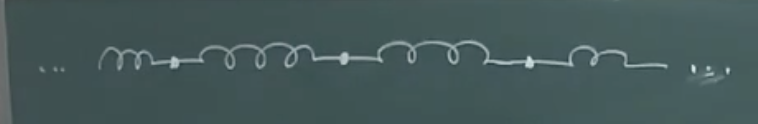
\includegraphics{img/1.png}
    \caption{一维经典弦示意图}
    \label{fig:my_label}
\end{figure}
为了简单起见,我们忽略了弹簧的质量,只考虑其提供的势能。假设初始时系统处于平衡态,相邻质点的距离为$l$,现在对弦的两端进行扰动,则弹簧会产生变形,每个质点相对于其平衡位置会产生偏离,我们记第$i$个质点偏离平衡位置的位移为$\eta_{i}$。
动能项$T=\frac{1}{2}\sum\limits_{i=1}\limits^{N}m\dot{\eta}_{i}^{2}$,势能项$V=\frac{1}{2}\sum\limits_{i=1}\limits^{N}k(\eta_{i+1}-\eta_{i})^{2}$。考虑连续极限(设总弦长为$L_{0}$是一固定的量,则有关系$L_{0}=Nl$,令$l\rightarrow0$,则$N\rightarrow \infty$),求和号变成积分,我们得到
\begin{equation}
    T=\frac{1}{2}\frac{m}{l}\sum\limits_{i}l\left(\frac{d\eta_{i}}{dt}\right)^{2}
    \rightarrow\frac{1}{2}\mu\int_{0}^{L_{0}}dx\left(\frac{\partial \eta(t,x)}{\partial t}\right)^{2}
\end{equation}
其中$\mu=\frac{m}{l}$代表弦的线密度。

类似地,我们有
\begin{equation}
    V=\frac{1}{2}kl\sum\limits_{i}l\left(\frac{\eta_{i+1}-\eta_{i}}{l}\right)^{2}
    \rightarrow\frac{1}{2}\tau\int_{0}^{L_{0}}dx\left(\frac{\partial \eta(t,x)}{\partial x}\right)^{2}
\end{equation}
其中$\tau=kl$代表弦的杨氏模量。

我们可以写出Lagrangian:
\begin{equation}
L=T-V=\int_{0}^{L_{0}}dx\left[\frac{1}{2}\mu\left(\frac{\partial \eta(t,x)}{\partial t}\right)^{2}-\frac{1}{2}\tau \left(\frac{\partial \eta(t,x)}{\partial x}\right)^{2}\right]
\end{equation}
其中,通常称
\begin{equation}
    \mathcal{L}=\frac{1}{2}\mu\left(\frac{\partial \eta(t,x)}{\partial t}\right)^{2}-\frac{1}{2}\tau \left(\frac{\partial \eta(t,x)}{\partial x}\right)^{2}
\end{equation}
为Lagrangian density,为了方便在不引起歧义的情况下也称为Lagrangian。
为方便,我们重新定义
$u(t,x)=\sqrt{\mu}\eta(t,x)$,则Lagrangian可重写为
\begin{equation}
\label{lagran}
L=T-V=\frac{1}{2}\int_{0}^{L_{0}}dx\left[\left(\frac{\partial \eta(t,x)}{\partial t}\right)^{2}-c^{2} \left(\frac{\partial \eta(t,x)}{\partial x}\right)^{2}\right]
\end{equation}
其中$c=\sqrt{\frac{\tau}{\mu}}$,为波速。与我们在理论力学里所做的事情相同,利用Euler-Lagrange方程,我们可以得到经典的波动方程。

我们接下来的任务是要量子化这个一维的经典场论。为了明确,我们假设弦的两端是固定的,即边界条件为$u(t,x=0)=u(t,x=l)=0$。下面我们把$u(t,x)$在位形空间做一个Fourier展开,得到
\begin{equation}
\label{fourier}
    u(t,x)=\sum\limits_{k=1}\limits^{\infty} q_{k}(t){\rm{sin}}\left( \frac{ \omega _{k} x}{c} \right)
\end{equation}
为了满足边界条件,正则角频率$\omega_{k}$必须满足离散条件$\omega_{k}=\frac{k\pi c}{L_{0}}$。
将(\ref{fourier})带回到(\ref{lagran}),并对$x$积分可以得到,
\begin{equation}
\label{fourierlag}
    L=\frac{L_{0}}{4}\sum\limits_{k=1}\limits^{\infty}\left\{\dot{q}_{k}^{2}(t)-\omega_{k}^{2}q_{k}^{2}(t)\right\}
\end{equation}
其Hamiltonian为
\begin{equation}
\label{hamil}
    H=\frac{L_{0}}{4}\sum\limits_{k=1}\limits^{\infty}\left\{\dot{q}_{k}^{2}(t)+\omega_{k}^{2}q_{k}^{2}(t)\right\}
\end{equation}
注意到单粒子在谐振子势下的Hamiltonian为
\begin{equation}
\begin{aligned}
    H&=\frac{\vec{p}^{2}}{2m}+\frac{1}{2}m\omega^{2}x^{2}\\
    &=\frac{1}{2}m\dot{x}^{2}+\frac{1}{2}m\omega^{2}x^{2}
    \end{aligned}
\end{equation}
因此可以发现(\ref{hamil})可以看作是无穷多个独立的谐振子的叠加\footnote{顺便一提,利用E-L方程可以从(\ref{fourierlag})中得到每个谐振子的运动方程$\ddot{q}(t)+\omega_{k}^{2}q_{k}=0$,其解可表示成$Ae^{-i\omega_{k}t}+Be^{i\omega_{k}t}$的形式}。对于一个单粒子谐振子系统,我们知道它的正则量子化方式将正则坐标与正则动量升级为算符并引入对易子$[\hat{x},\hat{p}]=i\hbar$。
对于我们现在所处理的一维弦,我们也可以采用类似的方式将其量子化。
定义正则动量
\begin{equation}
\label{canmomentum}
    p_{k}=\frac{\partial L}{\partial \dot{q}_{k}}=\frac{L_{0}}{2}\dot{q}_{k}(t)
\end{equation}
于是我们可以将Hamiltonian(\ref{hamil})重写为
\begin{equation}
\label{hamilnormal}
     H=H(p_{k},q_{k})=\sum\limits_{k=1}\limits^{\infty}\left\{\frac{p_{k}^{2}}{L_{0}}+\frac{L_{0}\omega_{k}^{2}}{4}q_{k}^{2}\right\}
\end{equation}
类比单谐振子的情况,引入等时量子化条件
\begin{equation}
\label{eqtime}
\begin{aligned}
    \left[\hat{p}_{i}(t),\hat{q}_{j}(t)\right]&=-i\hbar\delta_{ij}\\
    \left[\hat{q}_{i}(t),\hat{q}_{j}(t)\right]&=0\\
    \left[\hat{p}_{i}(t),\hat{p}_{j}(t)\right]&=0
    \end{aligned}
\end{equation}
其中$\hat{p}_{i},\hat{q}_{j}$都成为了算符。这样我们就实现了从经典场论到量子场论的转变。

在量子力学中,对于单粒子谐振子系统,我们可以在粒子数表象下将Hamiltonian写为
\begin{equation}
\label{danliziH}
    H=\hbar\omega(a^{\dagger}a+\frac{1}{2})
\end{equation}
其中有$\hat{x}\propto a+a^{\dagger},\;\hat{p}\propto i(a-a^{\dagger})$。在量子场论中我们想要做同样的事情,为此,考虑到在经典场论中$q_{k}$的解的形式应为$Ae^{-i\omega_{k}t}+Be^{i\omega_{k}t}$,以及$\hat{q_{k}}$应当是一个Hermite算符,因此我们将$\hat{q}_{k}$写成以下形式\footnote{值得注意的是在经典场论的情况下$q_{k}$的解在$e^{\pm i\omega_{k}t}$前的线性组合系数为普通的c-数,而在量子场论的情况下相应的位置变成了不对易的算符。}
\begin{equation}
\label{hermiteq}
\begin{aligned}
    \hat{q}_{k}(t)&=\sqrt{\frac{\hbar}{L_{0}\omega_{k}}}\left[a_{k}e^{-i\omega_{k}t}+a_{k}^{\dagger}e^{i\omega_{k}t}\right]\\
    \hat{p}_{k}(t)&=\sqrt{\frac{\hbar L_{0}\omega_{k}}{4}}\left[-a_{k}e^{-i\omega_{k}t}+a_{k}^{\dagger}e^{i\omega_{k}t}\right]
    \end{aligned}
\end{equation}
其中的时间依赖关系来自于经典情况的类比,系数$\sqrt{\frac{\hbar}{L_{0}\omega_{k}}}$类似于在单粒子的情况下$\hat{x}=\sqrt{\frac{\hbar}{2m\omega_{k}}}(a+a^{\dagger})$前的系数(由(\ref{canmomentum})可以看出相当于在单粒子的情况中取$m=\frac{L_{0}}{2}$),其中$a,\;a^{\dagger}$分别表示改变同一个粒子的量子数的下降和上升算符。类似地,在量子场论中我们称(\ref{hermiteq})中$a$为湮灭算符,可以湮灭一个量子,$a^{\dagger}$为产生算符,可以产生一个量子,根据之前的讨论,粒子是把场激发后对应的量子,因此(\ref{hermiteq})显式地表明了量子场论描述的是一个粒子数可变的系统。如果我们认为一维弦描述的是电磁场,则$a_{k},\;a_{k}^{\dagger}$分别湮灭和产生一个动量为$\vec{k}$光子。与在量子力学中的升降算符满足的对易关系$\left[a,a^{\dagger}\right]=1$,类似地,在场论中,量子化条件(\ref{eqtime})要成立,意味着有\footnote{可以试着代入检验一下}
\begin{equation}
    \begin{aligned}
    \left[a_{i},a^{\dagger}_{j}\right]&=\delta_{ij}\\
    \left[a_{i},a_{j}\right]&=0\\
    \left[a^{\dagger}_{i},a^{\dagger}_{j}\right]&=0
    \end{aligned}
\end{equation}
我们将(\ref{hermiteq})带入(\ref{hamilnormal})中可以得到用产生和湮灭算符得到的Hamiltonian为
\begin{equation}
    \label{hamila}
    \hat{H}=\sum\limits_{k=1}\limits^{\infty}\hbar \omega_{k}\left(a_{k}^{\dagger}a_{k}+\frac{1}{2}\right)
\end{equation}
这与单粒子情况(\ref{danliziH})非常相似,其差别在于无穷多频率的求和,这再次体现了量子场论是无穷多谐振子的联合,这一点在坐标空间并不是特别明显,可见在动量空间看问题有其独特的优越性。对于这一类Hamiltonian可以写成无穷多独立的谐振子的量子场论我们称之为自由场论,与之对应的是相互作用场论,顾名思义,自由场论是最简单的量子场论,而相互作用场论要复杂得多,不幸的是,描述自然界的场论都是含有相互作用的。

从(\ref{hamila})中我们可以到$H$中的每一项都含有$\frac{1}{2}$,这一项被称为零点能,其物理来源是著名的不确定性原理,在经典的情况下,当一个弹簧处于平衡位置时,我们可以同时确定位于弹簧末端的粒子的位置和速度,从而其动能和势能均为0,总能量为0;但是在量子力学中,由于我们无法同时确定这样一个粒子的位置和动量,因此导致在Hamiltonian中出现非零的效应。在量子场论中,零点能仍然来自于不确定性原理,但是其复杂性在于无穷多模式求和后,$\sum\limits_{k=1}\limits^{\infty}\frac{1}{2}\hbar \omega_{k}=\sum\limits_{k=1}\limits^{\infty}\frac{1}{2}\hbar \frac{k\pi c}{L_{0}}$ 是发散的,在量子场论中我们称其为真空能量,这是我们在量子场论中遇到的第一个无穷大。事实上,在量子场论中随处可见的无穷大也给这门课的学习造成了一定的困难,我们知道物理仪器只能够测量有限的物理量,因此这些数学上的无穷大是非物理的,那么如何处理这些无穷大是场论中十分引人入胜的一个课题,一般称之为重整化。

下面来讨论一维量子弦的能谱问题。对于单谐振子,我们知道$H\ket{0}=\frac{1}{2}\hbar \omega \ket{0}$,利用上升算符我们可以得到所有的激发态:$\ket{n}=\frac{(a^{\dagger})^{n}}{\sqrt{n!}}\ket{0}$。事实上我们有
\begin{equation}
    \begin{aligned}
    a\ket{n}&=\sqrt{n}\ket{n-1} \\
    a^{\dagger}\ket{n}&=\sqrt{n+1}\ket{n+1}
    \end{aligned}
\end{equation}
对于一维量子弦,情况是完全类似的,量子弦的本征态可以写为
\begin{equation}
    \ket{n_{1},n_{2},\cdots,n_{i},\cdots}
\end{equation}
其中$n_{k}$表示角频率为$\omega_{k}$模式的光子数,这是一个无穷维向量,因此哪怕我们要想刻画一个简单的一维量子弦系统,我们也必须使用无穷维的向量空间,为此我们引入一个广义的Hilbert空间,称之为Fock空间,Fock空间是一个无穷多个Hilbert空间的直和
\begin{equation}
\mathcal{F}=\bigoplus\limits_{n=1}\limits^{\infty}\mathcal{H}_{n}
\end{equation}
其中$\mathcal{H}_{n}$表示描述固定$n$个粒子的Hilbert空间,在非相对论量子力学中,我们通常只在一个固定的Hilbert空间$\mathcal{H}_{n}$内进行研究,但是在场论中会涉及到在不同Hilbert空间$\mathcal{H}_{n}$的转换。

\section{小结}
\begin{itemize}
    \item 场论中把谐振子的数学基本照搬了过来,但是其物理诠释做了相应改变,例如我们把谐振子中第$n$激发态$\ket{n}$诠释为有$n$个角频率为$\omega_{k}$的全同粒子的态。粒子和场是天然交织在一起的,粒子是场激发所对应的量子,粒子即量子。换句话说,量子场论给了波粒二象性一种非常具体的实现方式。
    \item 量子化后弦的真空能是无穷多零点能的和,是一个发散的量。这是一个非常普遍的现象,对于几乎所有的量子场论而言其真空能都是发散的。发散的量不对应直接的物理可观测量,为了处理这种发散的量,我们需要重整化的概念。
    \end{itemize}
    
    顺便提一下历史上量子场论的后续发展,1927年Dirac成功量子化电磁场并推导了正确的原子自发辐射公式之后\footnote{Einstein根据热力学的方法最早得出了正确的单原子的自发辐射公式},很快Heisenberg和Pauli在1929年引入了量子场论的正则量子化框架\footnote{所谓正则量子化就是我们上面对一维弦所做的量子化流程,引入正则坐标与正则动量的对易关系来实现量子化的目的。在这门课中我们只涉及正则量子化。},量子化了K-G场以及Dirac场。可以这样认为,在1920年代末期,量子场论的框架已经成立了,在1930年代人们通过电子自能认识到了场论中的无穷大的存在,1947年,在我们之前提到过的Shelter Island Conference,Schwinger、Feynman等人发展了QED,成功解释了电子反常磁矩和Lamb位移。在此过程中,重整化理论也比较成熟地发展了起来。随后在1967-1973年,基于$SU(3)\times SU(2)\times U(1)$规范场论的标准模型建立,这个模型只有20个左右手放的参数,但可以预言当时几乎所有的高能物理现象,标准模型是20世纪人们在自然科学领域的伟大成就。1972年K.Wilson提出了重整化群的概念,用于解释二阶相变的普适性等问题,这一概念也深刻地影响了其他的物理分支,如凝聚态物理等。
